\section{Causal-window California backtests and JMA trend ablation}

\label{sec:s06-completed}

The California and JMA values in this section are recovered original fit and score outputs with checked hashes and source identities. The fitting and rescoring described below belong to the original study; this edition does not recompute them. The original audit coverage is retained.

The completed California map contains five eligible episodes, in 1994, 1999, 2004, 2010 and 2019. The two 1992 episodes are excluded by the predeclared training-count or zone-adequacy rule, not silently replaced by a more favourable sequence. Training expands from 1986 up to, but not including, each episode origin; the parent history retains the 1981 warmup. Each scored block ends at the earlier of the next eligible origin, one year after its origin, or the coverage cutoff. Parameters, spatial scale and nuisance inputs are selected only on the preceding training prefix.

The $M\geq6$ episode origins were identified retrospectively from the catalogue. The roster is retrospective and exploratory. Overlapping training histories and a common archive mean that the five episodes are not independent replications. The active partition is the union of declared episode time intervals, and its complement fills the rest of the scored block; it does not causally label individual earthquakes as aftershocks.

\begin{table}[htbp]\centering\caption{Held-out joint scores (nats) on the five eligible California blocks. Higher is better. These descriptive scores have no confidence intervals.}\label{tab:s06-ca}

\begin{tabular}{lrrrrr}\toprule Year & Targets & FC & MC & OC & EP\\\midrule

1994 & 64 & -527.0462 & -525.5013 & -526.7452 & -521.5603 \\

1999 & 75 & -551.4448 & -545.6841 & -540.1365 & -521.8412 \\

2004 & 30 & -349.2570 & -347.5086 & -347.8333 & -341.1560 \\

2010 & 125 & -1044.6385 & -1055.3761 & -1050.2614 & -1059.1042 \\

2019 & 127 & -696.3825 & -679.3514 & -670.2133 & -647.9267 \\

\bottomrule\end{tabular}\end{table}

\begin{table}[htbp]\centering\caption{OC minus FC joint contrasts, partitioned without changing fitted parameters. Full equals active plus complement, subject to the saved numerical tolerance. These contrasts are descriptive; no confidence intervals are supplied.}

\begin{tabular}{lrrrrr}\toprule Year & Active $N$ & Complement $N$ & Full & Active & Complement\\\midrule

1994 & 49 & 15 & 0.3010 & -0.0672 & 0.3682 \\

1999 & 61 & 14 & 11.3083 & 11.3970 & -0.0887 \\

2004 & 7 & 23 & 1.4237 & -0.1897 & 1.6134 \\

2010 & 75 & 50 & -5.6229 & -6.0147 & 0.3918 \\

2019 & 111 & 16 & 26.1693 & 26.3067 & -0.1374 \\

\bottomrule\end{tabular}\end{table}

EP achieves the highest held-out joint score in the 1994, 1999, 2004 and 2019 blocks, but loses in the 2010 block. That block contains 125 targets: 75 active and 50 in the complement.

EP's joint score of -1059.1042 is below OC (-1050.2614), FC (-1044.6385) and MC (-1055.3761). OC also trails FC: its joint contrast is -5.6229 nats, comprising -6.0147 active nats and 0.3918 complement nats. EP's joint advantage in the three primary chronological folds is therefore not uniform across every retrospective episode block.

The 2019 episode block contains 127 targets (111 active and 16 in the complement). It starts at the $M\geq6$ episode origin and runs for one year, so its denominator differs from the UTC calendar-2019 slice in Section~\ref{sec:calendar-sequence-partition}.

For JMA, the free-trend states are the preserved training-selected parameters, rescored without gratuitous refitting. The stationary alternative fixes $d=0$ and refits the prescribed starts and floors under the same training nuisance inputs. Both trends use identical target populations, the reported magnitude-lattice counting measure and all 1,277 targets across the three folds.

\begin{table}[htbp]\centering\caption{JMA contrasts (nats) under free and stationary background trend. Positive values favour OC. These contrasts are descriptive; no confidence intervals are supplied.}\label{tab:s06-jma}

\begin{tabular}{llrrrr}\toprule Fold & Trend & Targets & OC--FC timing & OC--EP timing & OC--EP joint\\\midrule

0 & free & 469 & -19.9765 & -1.1943 & -74.7591 \\

0 & $d=0$ & 469 & -20.0603 & -5.8012 & -76.4264 \\

1 & free & 348 & -12.8718 & -1.4445 & -59.1334 \\

1 & $d=0$ & 348 & -8.1665 & -4.1719 & -61.1146 \\

2 & free & 460 & -25.7452 & -5.0868 & -87.3190 \\

2 & $d=0$ & 460 & -9.6847 & -3.6114 & -84.6859 \\

\midrule

All & free & 1277 & -58.5935 & -7.7256 & -221.2115 \\

All & $d=0$ & 1277 & -37.9115 & -13.5846 & -222.2269 \\

\bottomrule\end{tabular}\end{table}

These ablation contrasts diagnose sensitivity to the fitted trend within the declared procedures. They do not isolate a physical mechanism, certify global optimization, or establish independent cross-region validation. Saved acceptance checks cover source and cache identities, causal windows, retained parent prefixes, required start/floor coverage, selected parameter reuse, numerical refinement, proper-score identities and the complete temporal partition. No independent likelihood replay is claimed by this completion check.

Fixing the background trend at zero reduces the pooled OC--FC timing deficit but does not eliminate it. The OC--EP joint deficit also persists, so a lower-bound trend estimate alone does not explain the Japanese reversal.

New Zealand remains an adaptively reused archive in this manuscript. S06 supplies no fresh New Zealand cohort and does not remove the adaptive-reuse disclosure or the need for genuinely prospective validation.

\begin{figure}[htbp]\centering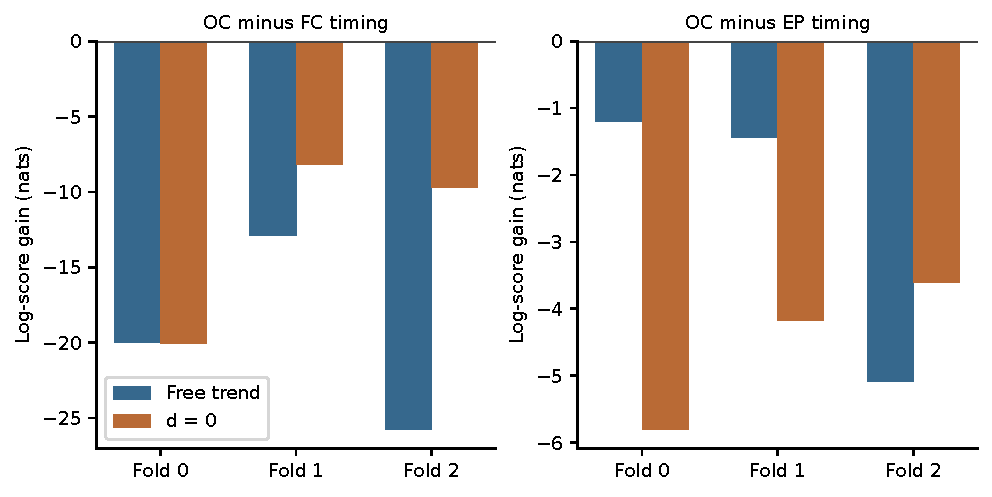
\includegraphics[width=\textwidth]{s06_jma_trend_timing.pdf}\caption{Saved JMA timing contrasts under free and stationary background trends. Each bar uses the same fold population; no new likelihood calculation or simulation was performed for the plot.}\end{figure}
